\documentclass{tufte-handout}
\usepackage{booksprint}

\title[SDA2 -- Integration in Strategic DDD]{SDA2 -- Integration Patterns in Strategic Domain Driven Design}
\author{Sebastian Höhn}
\date{\today}

\begin{document}
\maketitle
\logos

\section{Introduction}
In the lecture we have discussed the the concept of domains and sub-domains
as well as the \textit{bounded context} in strategic domain driven design. 
The bounded contexts can be arranged in a hierachy-like structure\footnote{Remember that
some contexts my be upstream and downstream at the same time and the resulting
dependency graph might not be a tree or not even be free of cycles. If your dependency graph
becomes overly complex think about re-designing it.}. 

The idea behing integration patterns is to define a set of best practices on how we
control upstream and downstram behaviour in context dependencies.

This short paper presents a list of patterns. For further details check the book 
by~\citet{Khononov2022}.

\section{Cooperation Patterns}

These patterns require well-established communication between the teams that
develop and maintain the contexts. They might even be developed in the same team.

\subsection{Partnership}

Coordination happens in an ad hoc way. One team notfies the other about changes in 
the context and the other team will cooperat and adapt. There is no team in the lead
for changes, it works in both ways. Each team can initiate a change. It is important 
that they cooperate in soving integration issues and that no team is interested in
blocking the integration.

\begin{figure}
    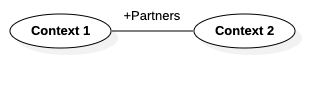
\includegraphics[width=.8\textwidth]{img/integrating_context_partners.png}
    \caption{Modeling partnership in bounded contexts.}
\end{figure}

\subsection{Shared Kernel}

Although we always claim that the bounded contexts are also model boundaries, you will 
frequently encounter situations where the same model is part of different subdomains and
hence the respective bounded context. In such a case these shared models must be consistent
in all the  bounded contexts!

A typical example of such a model is Identity and Access Management. This is rarely a core
domain, but the identities used throughout your bounded contexts should always be the same 
(say single sign on). In such a case each user might have permissions originating in different
domains. Furthermore, each domain might have special requirements regarding the IAM.

It is obviuos that a \textit{shared kernel} creates a thight coupling between the domains.
Changes in the shared models must immediately be reflected in all subdomains. Hence we 
need to implement mechanisms for continuous integration to technically solve that dependency.

The pattern is a trade-off between the \textit{cost of duplication} vs the 
\textit{cost of coordination}. Discussing the trade-off is beyond the scope of this 
short introduction of the patterns, but consider the example of single-sign-on.

\begin{figure}
    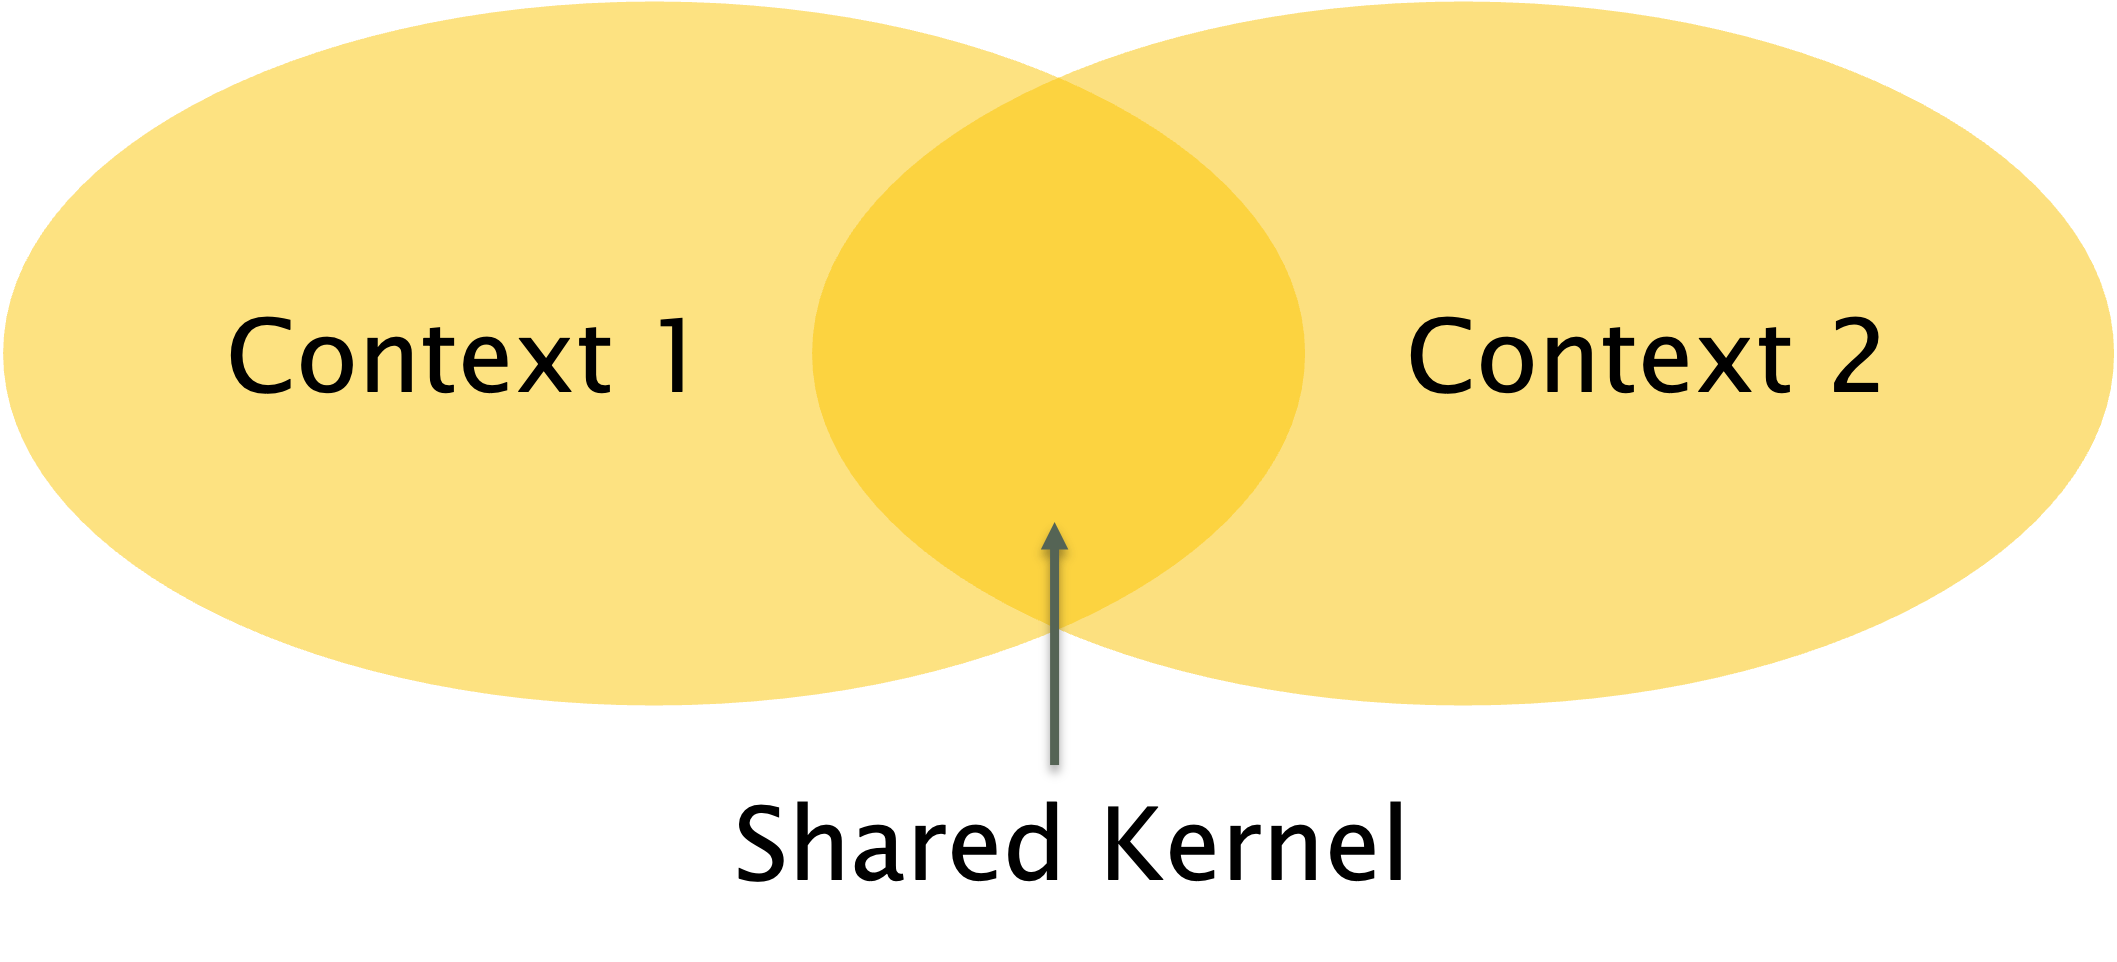
\includegraphics[width=.8\textwidth]{img/integrating_context_shared_kernel.png}
    \caption{Modeling shared kernels in bounded contexts.}
\end{figure}

\section{Customer-Supplier Patterns}

This set patterns define a type of hierarchy. The supplier provides a service to the 
customers. The supplier is upstream and the customer downstream (i.e. the customer
receives the issue from the supplier).

\subsection{Conformist}

This pattern is in favor of the upstream team. It just provides the integration contract,
which is defined according to the upstream model (take it or leave it). That means that
the downstream customer must conform to the integration provided.

There are several reasons to follow that pattern. It might just be organzational governance
or necessities arising from external suppliers: the contract might be an industry standard
or another well-established model (e.g. ERP-System, cloud solution or Software as a Service
Integration).

\begin{figure}
    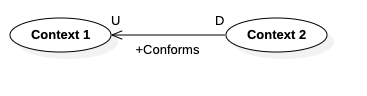
\includegraphics[width=.8\textwidth]{img/conforms.png}
    \caption{Modeling the conformist patter in bounded contexts.}
\end{figure}

Do not forget: in some cases it might just be good enough for your concrete situation. And 
everything else might be more expensive (compare to the principle \textit{"buy before make"}).

\subsection{Anticorruption Layer}

This pattern also assumes, that changes in upstream contexts can happen. In this case it
is not agreed upon the idea that the context will be able to conform. Therefore, it will
translate the upstream bounded context model into a customized model for its own context.
The translation is implemented in the \textit{anticorruption layer}.

\begin{figure}
    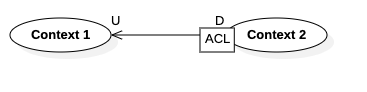
\includegraphics[width=.8\textwidth]{img/anticorruption.png}
    \caption{Modeling the anticorruption layer in bounded contexts.}
\end{figure}

Criteria for the decision when you might want to implement such a layer might be:

\begin{itemize}
    \item The customer's context contains a core subdomain
    \item The supplier's model is inefficient for the consumer needs
    \item The supplier's model changes too frequently
\end{itemize}

\subsection{Open-Host Service}

This pattern is the opposite of the anticorruption layer. The supplier protects the 
consumers by implementing an \textit{open-host service} which decouples the public
interface from the implementation and thus allows for the implementation and evolution
of both in different timelines.

\begin{figure}
    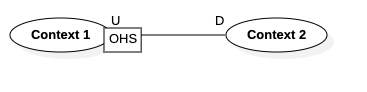
\includegraphics[width=.8\textwidth]{img/openhost.png}
    \caption{Modeling open-host service pattern in bounded contexts.}
\end{figure}

The advantage is that the supplier's public interface (i.e. open-host service) must not
conform to its ubiquitous language. It can furthermore be translated into an integration
oriented language. This language is called the \textit{published language}.

This pattern allows to provide multiple versions of published languages to be provided
for different consumers.

\begin{figure}
    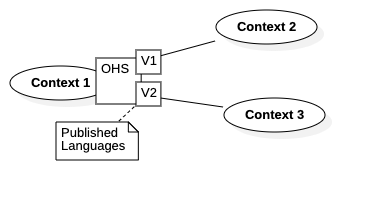
\includegraphics[width=.8\textwidth]{img/multi-ohs.png}
    \caption{Muliple published languages implementes with the open-host service pattern.}
\end{figure}

\section{Separate ways}

In this short paper we have discussed collaboration patterns for strategic domain
driven design. To cope with the ubiquitous trade-off in architecture decisions
it is important to mention that \textit{the decision to not collaborate is a 
valid option}, too. It may just be more cost-efficient to go separate ways and
duplicate functionality in multiple bounded contexts.

Criteria for such a decision might be:

\begin{itemize}
    \item \textit{Generic Subdomains:} the solution is generic, and it is easy to integrate
    it is normally more cost-effective to integrate it locally (imagine a logging 
    service)
    \item \textit{Communication issues:} due to size of the company or internal policies
    collaboration might be to costly.
    \item \textit{Model Differences:} models may be so different that a conformist relationship
    is not possible. Furthermore, an anticorruption layer might become more complex
    than duplicating the functionality.
\end{itemize}

% The bibliography style.
\bibliographystyle{apalike}

% If you DO want the full list of references to be printed at the end.
\bibliography{references}

% If you do NOT want the full list of references to be printed at the end.
%%\nobibliography{references}

\begin{figure}
    
\includegraphics[width=2cm,right]{img/cc-by.png}
\end{figure}

\end{document}